\chapter{Research and Planning} \label{Research and Planning}

\section{Product Development Process}

\begin{enumerate}
    \item \textbf{Research Phase}
    
           \noindent Initial stage, knowing what we have, what we want           and where to get that. Research on current products available in the market, survey on the customer needs and study on different designs and materials.
          
    \item \textbf{Conceptual Design Stage}
    
           \noindent Series of organised concepts of concise design              based on the research done. Selecting the best design out of multiple concepts, based on multiple factors such as manufacturability, reliability.
           
    \item \textbf{Design Evaluation}
    
           \noindent Evaluating the conceptual design in stress         analysis and CAD software to look for disabilities. Improving the design and eliminating all the shortcomings.
           
    \item \textbf{Design FMEA}
    
            \noindent Failure mode effect analysis of the design to prioritize the risk of different failure modes.
            
    \item \textbf{Monitoring Progress}
    
           \noindent Keeping logs of all activities. Maintaining a project diary to keep track of all the activities done, outcomes of meetings and project stages, to keep a progress check and quickly refer to all the various tasks done.
           
    \item \textbf{Prototyping}
     
           \noindent Fabricating a prototype based on the project design to understand it's interaction in the real world.
           
    \item \textbf{Testing}
    
           \noindent Simulated and real world testing on the prototype to make sure the project works as intended.
           
\end{enumerate}
\pagebreak

\section{Field Visit}
\noindent To learn about the techniques which are currently used to collect cow dung in a cow shed we visited Akhil Vishva Jai Shri Ram Gosanvardhan Kendra, Valpoi and interacted with people who regularly have to collect large amount of cow dung.

\begin{figure}[H]
  \centering
    \begin{minipage}{0.40\textwidth}
    \centering
      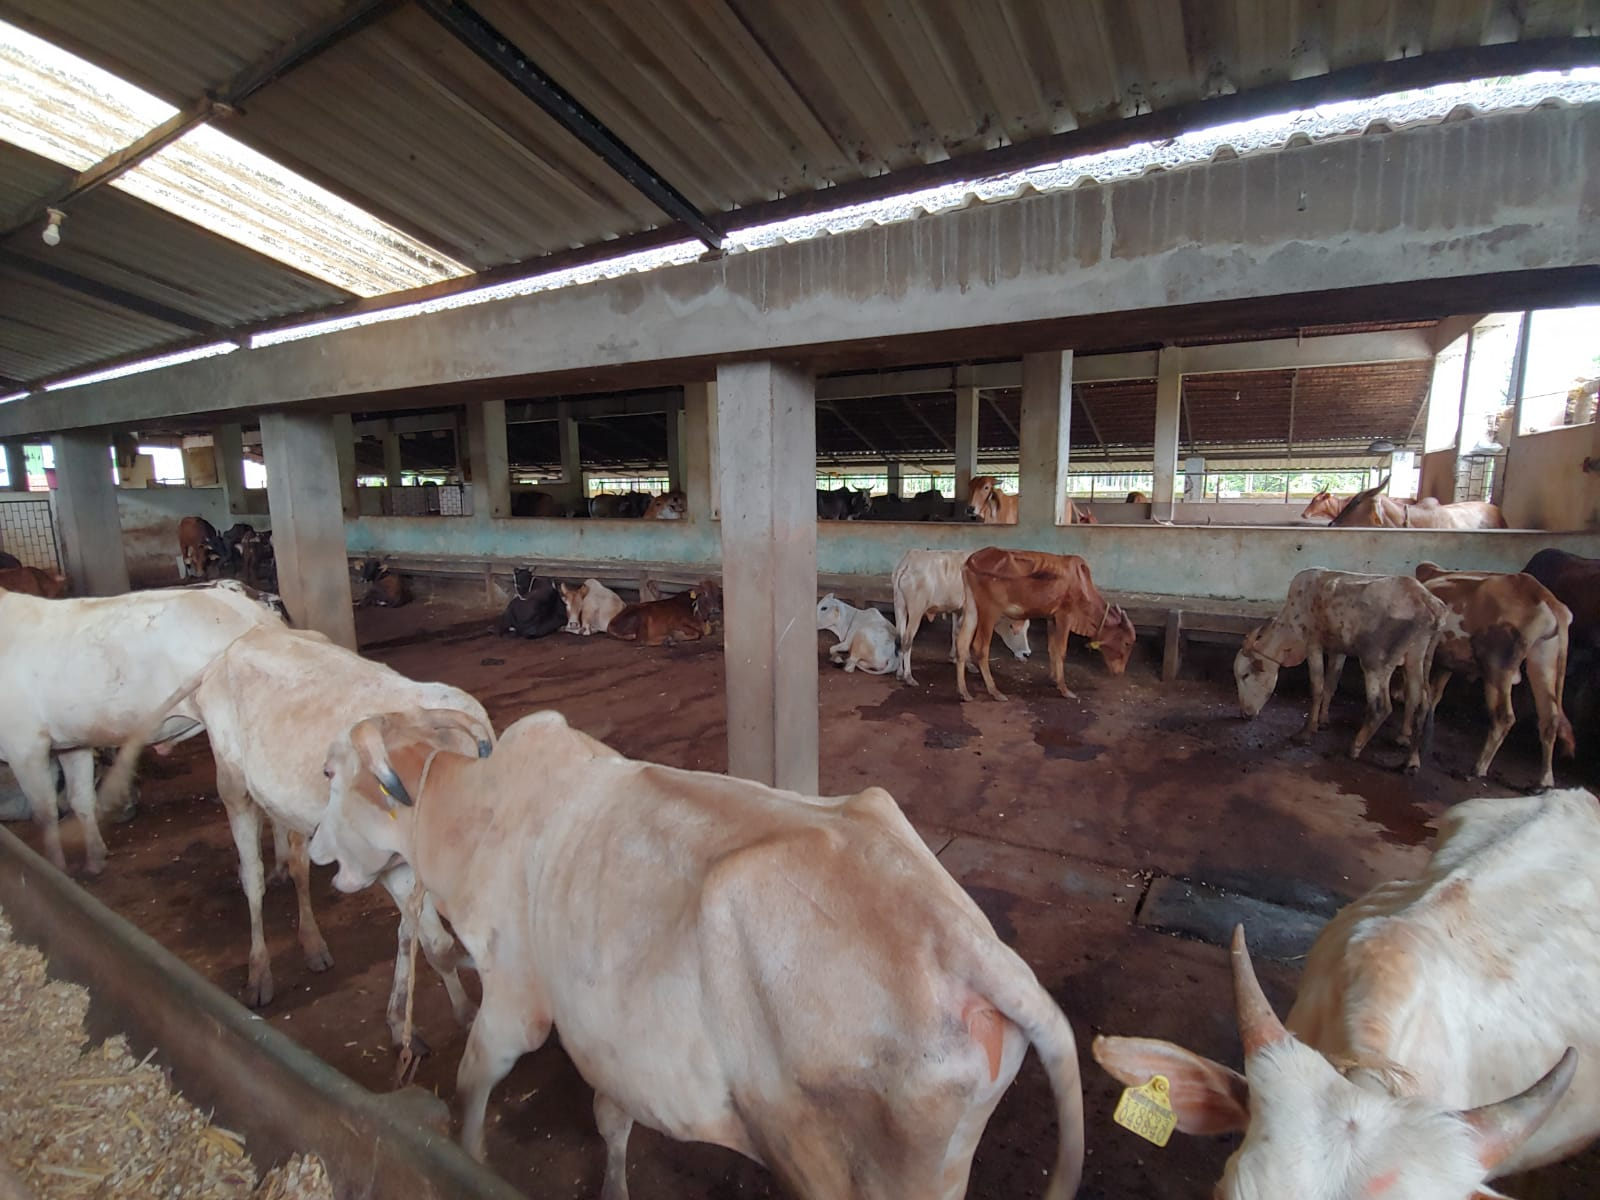
\includegraphics[width=1\textwidth]{Cow Shed.jpg}

    \end{minipage}
\hfill
    \begin{minipage}{0.40\textwidth}
    \centering
      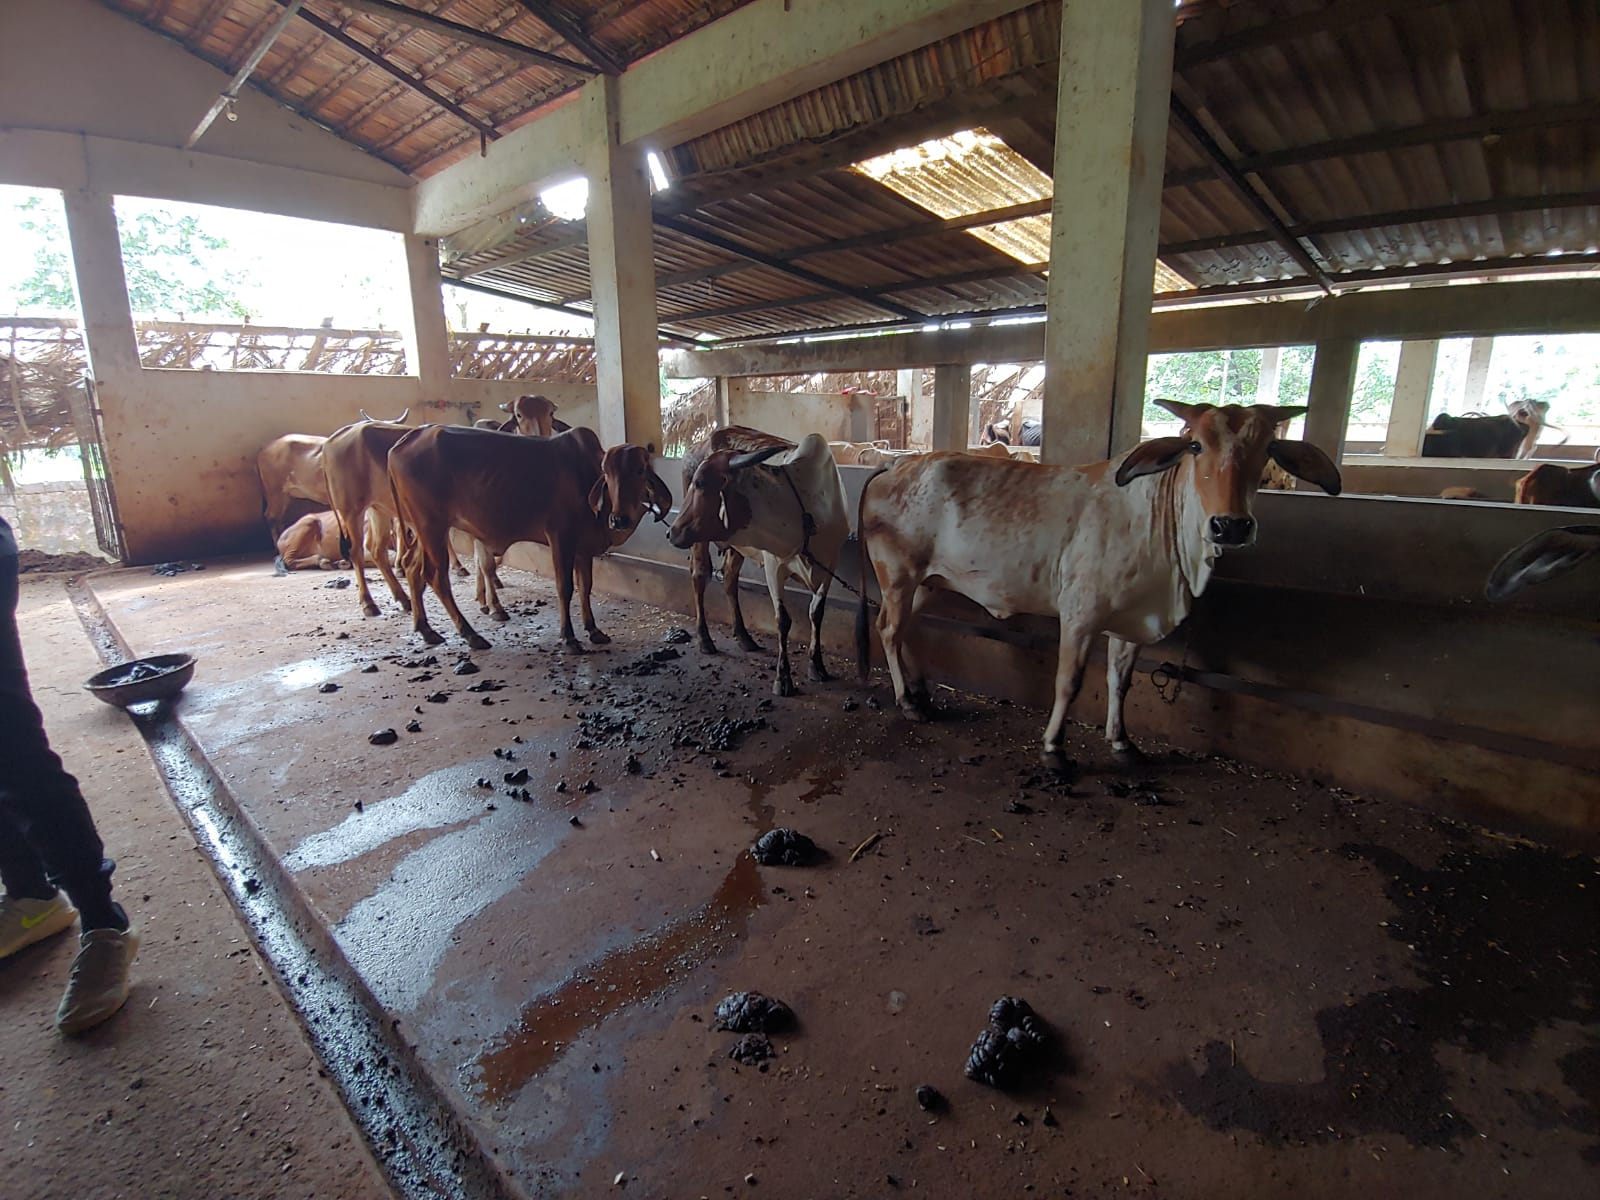
\includegraphics[width=1\textwidth]{Cow Shed 2.jpg}

    \end{minipage}
\caption{Cow Shed}
\end{figure}



\noindent We learnt that usually in cow sheds people collect cow dung twice a day and it is a very tiring and time consuming process. Cow dung is collected with the help of utensil (Fig. \ref{fig:Utensil}) by the worker and put in a large trolley. (Fig. \ref{fig:Trolley})Once the trolley is filled completely, it is emptied at the nearby dumping ground. 

\begin{figure}[H]
  \centering
    \begin{minipage}{0.35\textwidth}
    \centering
      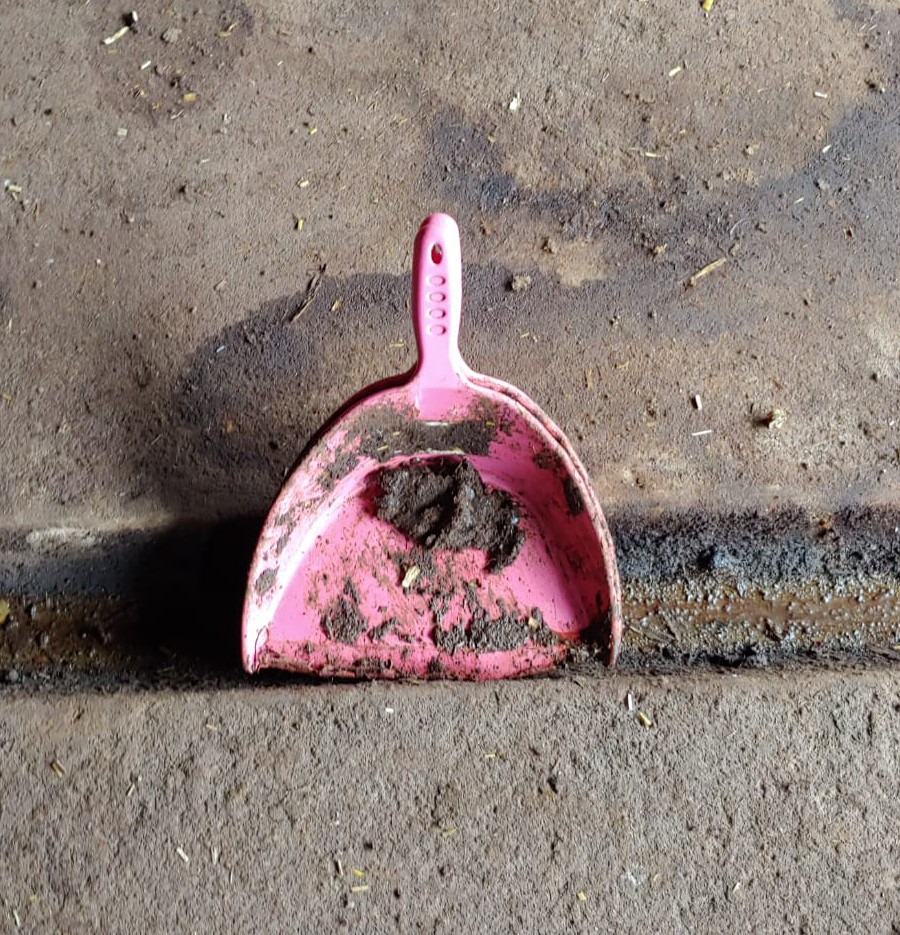
\includegraphics[width=0.9\textwidth]{Utensil.jpg}
      \caption{Utensil}
      \label{fig:Utensil}
    \end{minipage}
    \begin{minipage}{0.40\textwidth}
    \centering
      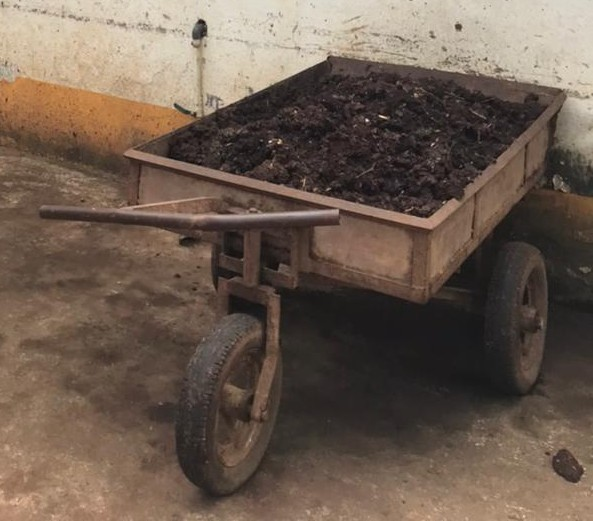
\includegraphics[width=0.9\textwidth]{Trolley.jpg}
      \caption{Trolley}
      \label{fig:Trolley}
    \end{minipage}
\end{figure}

\noindent After communicating with the workers and manager of the farm we noted the following difficulties faced by them.
\begin{itemize}
    \item Poor hygiene conditions for the cow dung collecting workers.
    
    \item More labour being needed to be hired by the owners of the farm as cow dung collection by present method is very time consuming.

     \item Present method is very energy intensive and the workers often experience body fatigue due to constant bending in order to collect the cow dung.
     
\end{itemize}

\noindent They expected following attributes from a cow dung collecting machine.

\begin{itemize}
    \item Faster and easier to collect cow dung.
    \item Highly cost effective then the present machines available.
    \item Robust design to make sure it can be utilized in all sorts of terrains.
    \item At least 30 kg of collection capacity.
    
\end{itemize}

\pagebreak





\section{Design For Manufacturability}

\begin{itemize}

\item The general practice of designing products in a way that they        are easy to manufacture. This will help us design a product at       a very competitive cost by improving its manufacturability.

\item This will benefit us as our product will be simple to produce,       low in cost and will have improved reliability.

\item The functions of DFM which will be implemented in our product        are

      \begin{enumerate}
         
       \item The process selection decisions will be taken        accordingly based on our design to achieve a very cost-effective manufacturing.

       \item Will be able to estimate our manufacturing costs based on the selected processes.

       \item We will evaluate the design features for manufacturability in a CAD system by making solid models.
       
       \end{enumerate}
       
\end{itemize}